\newif\ifglobal

%%%%%%%%%%%%%%%%%%%%%%%
%%% Compile to view %%%
%%%%%%%%%%%%%%%%%%%%%%%

%%%%%%%%%%%%%%%%%%%%%%%%%%%%%%%%%%%%%%%%%%%%%%%%%%%
%%% Readme:                                     %%%
%%% https://www.overleaf.com/read/bwdjvfjksvjy/ %%%
%%%%%%%%%%%%%%%%%%%%%%%%%%%%%%%%%%%%%%%%%%%%%%%%%%%

% >>> M?: marks a module setting number or important notice

% >>> M4: Set {./relative-path} to external files for this module <<<
\def \modulefiles {./27-SDHOST}
% To add an external file, use:
% (Replace '---' with actual filename)
% '\input{\modulefiles/tables/---.tex}' for tables
% '\includegraphics{\modulefiles/figures/---}' for figures
% '\subfile{\modulefiles/---}' for register files

% >>> M1: This module is in global project? <<<
% 'YES' - uncomment; 'NO' - comment out
\globaltrue

\ifglobal
    \documentclass[main\_\_EN.tex]{subfiles}

\else
    \documentclass[openany, 10pt]{book}

    % >>> M2: In ./00-shared/preamble-trm-module, also find
    %         settings for visibility of todo notes, watermark <<<
    \usepackage{preamble-trm-module}

    % >>> M3: Temporary labels in English,
    %         you can add your own labels there <<<
    \myexternaldocument{./00-shared/temp-labels-en}

\fi %\ifglobal


\setcounter{secnumdepth}{4}


% >>> M5: If this module needs any updates in
% './00-shared/preamble-trm-module.sty'
% (include additional package, etc.), contact your module PM
% or create the file './00-shared/changelog.tex' make the
% necessary updates yourself and document them in this file <<<

% Make text left-aligned and allow latex to break pages naturally, comment out for full justification
\raggedright
\raggedbottom


\begin{document}


% Sets language into which pre-defined bits of text are translated
\selectlanguage{english}
\setenglishformatting

% Do not delete this block
\ifglobal
% Add the following front matter if
% this module is outside of global project
\else
    \InputIfFileExists{readme}{}{}
    \listoftodos
    {\let\clearpage\relax \listofdonetodos}
    \tableofcontents
    %\listoftables
    %\listoffigures
\fi


%%%%%%%%%%%%%%%%%%%%%%%%%
%%% TRM Module Begins %%%
%%%%%%%%%%%%%%%%%%%%%%%%%

\hypertarget{sdhost}{}
\chapter{SD/MMC Host Controller (SDHOST)}
\label{mod:sdhost}

\section{Overview}

The ESP32 memory card interface controller provides a hardware interface between the Advanced Peripheral Bus (APB) and an external memory device. The memory card interface allows the ESP32 to be connected to SDIO memory cards, MMC cards and devices with a CE-ATA interface. It supports two external cards (Card0 and Card1).

\section{Features}
This module has the following features:
\begin{itemize}
    \item Two external cards
    \item Supports SD Memory Card standard: versions 3.0 and 3.01
    \item Supports MMC: versions 4.41, 4.5, and 4.51
    \item Supports CE-ATA: version 1.1
    \item Supports 1-bit, 4-bit, and 8-bit (Card0 only) modes
\end{itemize}
The SD/MMC controller topology is shown in Figure \ref{Figure:card_system_topo}.
The controller supports two peripherals which cannot be functional at the same time.

\begin{figure}[H]
    \centering
    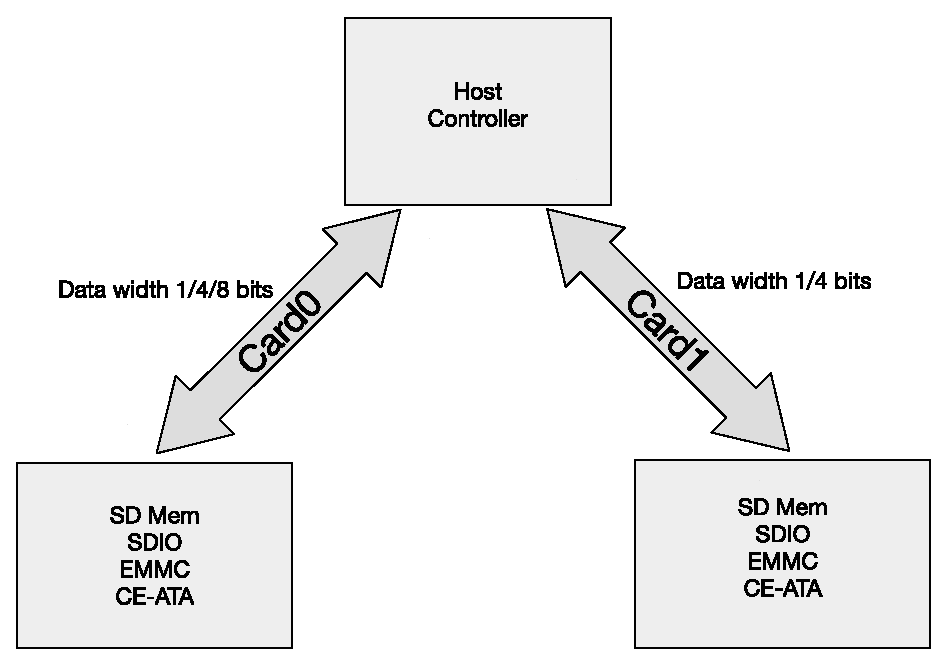
\includegraphics[width=0.55\textwidth]{./27-SDHOST/figures/cardsystemtopo.eps}
    \caption{SD/MMC Controller Topology}
    \label{Figure:card_system_topo}
\end{figure}

\section{SD/MMC External Interface Signals}
The primary external interface signals, which enable the SD/MMC controller to communicate with an external device, are clock (clk), command (cmd) and data signals. Additional signals include the card interrupt, card detect, and write-protect signals. The direction of each signal is shown in Figure \ref{Figure:SDIO_HOST_IF}. The direction and description of each pin are listed in Table \ref{SDMMC Signal Description}.

\begin{figure}[H]
    \centering
    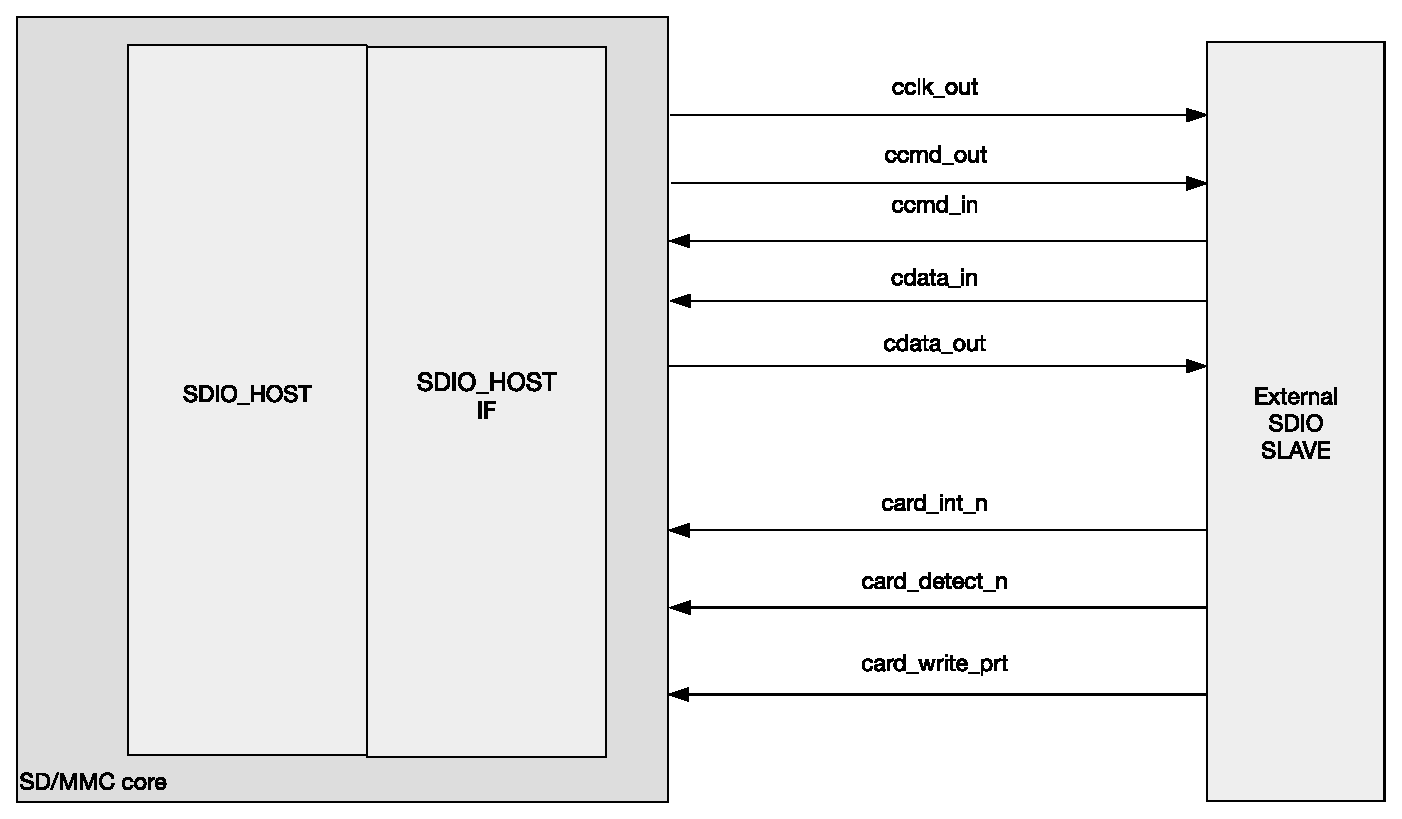
\includegraphics[width=0.7\textwidth]{./27-SDHOST/figures/SDIO_HOST_IF}
    \caption{SD/MMC Controller External Interface Signals}
    \label{Figure:SDIO_HOST_IF}
\end{figure}

\begin{longtable}[c]{ |p{3cm}|p{4cm}|p{8cm}| }
\caption{SD/MMC Signal Description} \label{SDMMC Signal Description}\\
\hline
\rowcolor{lightgray}
Pin & Direction & Description \\
\hline
\endfirsthead
\hline
\rowcolor{lightgray}
Pin & Direction & Description  \\
\hline
\endhead
\endfoot
cclk\_out & Output & Clock signals for slave device	\\\hline
ccmd & Duplex & Duplex command/response lines  \\\hline
cdata & Duplex & Duplex data read/write lines	\\\hline
card\_detect\_n & Input &  Card detection input line\\\hline
card\_write\_prt & Input & Card write protection status input 	\\\hline
\end{longtable}

\section{Functional Description}
\subsection{SD/MMC Host Controller Architecture}
The SD/MMC host controller consists of two main functional blocks, as shown in Figure \ref{Figure:SDIO_HOST_block_diagram}:

\begin{itemize}
    \item Bus Interface Unit (BIU): It provides APB interfaces for registers, data read and write operation by FIFO and DMA.
    \item Card Interface Unit (CIU): It handles external memory card interface protocols. It also provides clock control.
\end{itemize}

\begin{figure}[H]
    \centering
    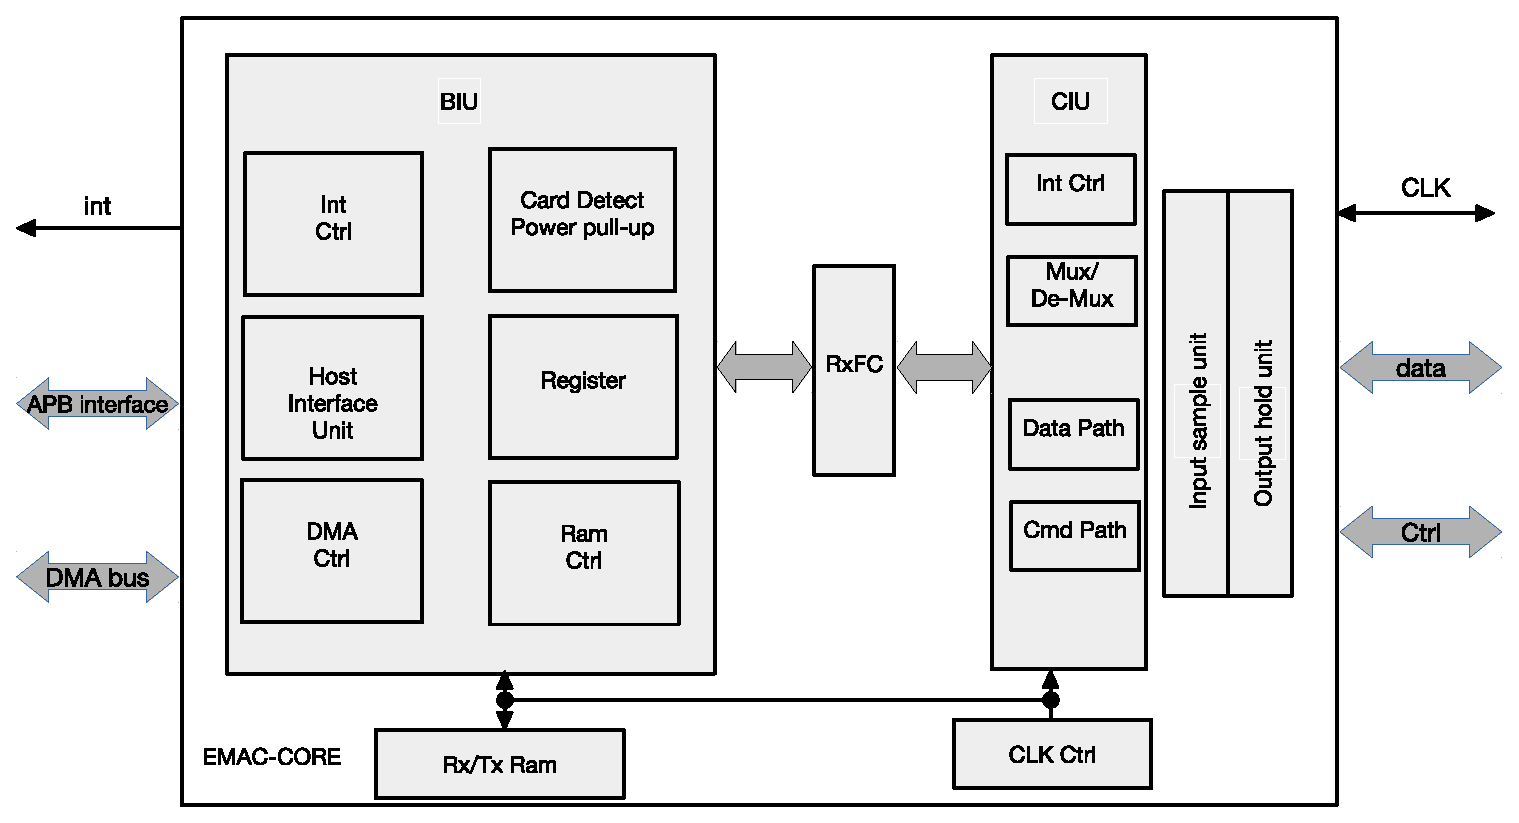
\includegraphics[width=0.7\textwidth]{./27-SDHOST/figures/SDIO_HOST_block_diagram}
    \caption{SDIO Host Block Diagram}
    \label{Figure:SDIO_HOST_block_diagram}
\end{figure}

\subsubsection{BIU}
The BIU provides the access to registers and FIFO data through the Host Interface Unit (HIU). Additionally, it provides FIFO access to independent data through a DMA interface. The host interface can be configured as an APB interface. Figure \ref{Figure:SDIO_HOST_block_diagram} illustrates the internal components of the BIU. The BIU provides the following functions:

\begin{itemize}
	\item Host interface
	\item DMA interface
	\item Interrupt control
	\item Register access
	\item FIFO access
	\item Power/pull-up control and card detection
\end{itemize}

\subsubsection{CIU}
The CIU module implements the card-specific protocols. Within the CIU, the command path control unit and data path control unit prompt the controller to interface with the command and data ports, respectively, of the SD/MMC/CE-ATA cards. The CIU also provides clock control. Figure \ref{Figure:SDIO_HOST_block_diagram} illustrates the internal structure of the CIU, which consists of the following primary functional blocks:

\begin{itemize}
	\item Command path
	\item Data path
	\item SDIO interrupt control
	\item Clock control
	\item Mux/demux unit
\end{itemize}

\subsection{Command Path}
The command path performs the following functions:

\begin{itemize}
	\item Configures clock parameters
	\item Configures card command parameters
	\item Sends commands to card bus (ccmd\_out line)
	\item Receives responses from card bus (ccmd\_in line)
	\item Sends responses to BIU
	\item Drives the P-bit on the command line
\end{itemize}

The command path State Machine is shown in Figure \ref{Figure:cmd_state_machine}.


\begin{figure}[H]
    \centering
    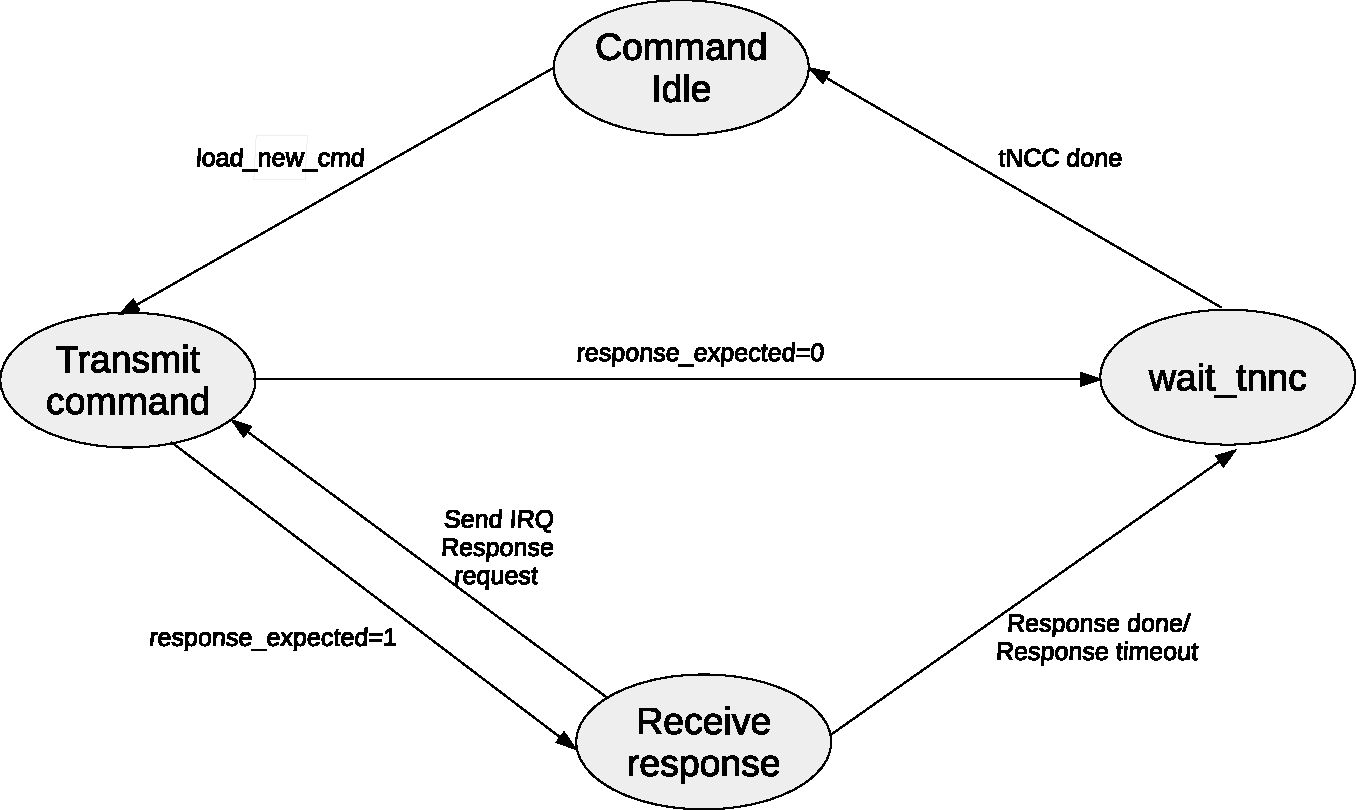
\includegraphics[width=0.5\textwidth]{./27-SDHOST/figures/cmd_state_machine}
    \caption{Command Path State Machine}
    \label{Figure:cmd_state_machine}
\end{figure}

\subsection{Data Path}

The data path block pops FIFO data and transmits them on cdata\_out during a write-data transfer, or it receives data on cdata\_in and pushes them into FIFO during a read-data transfer. The data path loads new data parameters, i.e., expected data, read/write data transfer, stream/block transfer, block size, byte count, card type, timeout registers, etc., whenever a data transfer command is not in progress.

If the data\_expected bit is set in the Command register, the new command is a data-transfer command and the data path starts one of the following operations:

\begin{itemize}
\item Transmitting data if the read/write bit = 1
\item Receiving data if read/write bit = 0
\end{itemize}

\subsubsection{Data Transmit Operation}

The data transmit state machine is illustrated in Figure \ref{Figure:tx_data_state_machine}. The module starts data transmission two clock cycles after a response for the data-write command is received. This occurs even if the command path detects a response error or a cyclic redundancy check (CRC) error in a response. If no response is received from the card until the response timeout, no data are transmitted. Depending on the value of the transfer\_mode bit in the Command register, the data-transmit state machine adds data to the card's data bus in a stream or in block(s).
The data transmit state machine is shown in Figure \ref{Figure:tx_data_state_machine}.

\begin{figure}[H]
    \centering
    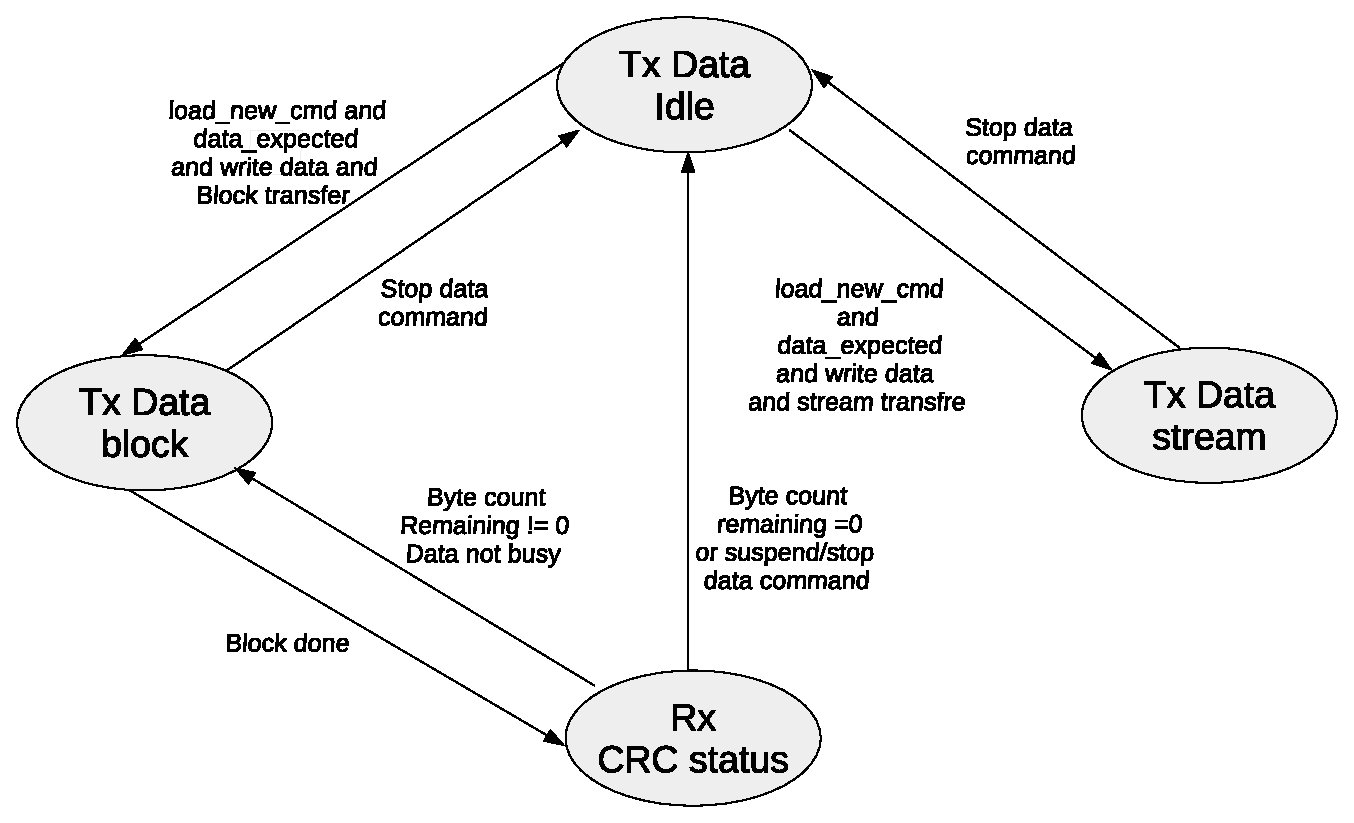
\includegraphics[width=0.5\textwidth]{./27-SDHOST/figures/tx_data_state_machine}
    \caption{Data Transmit State Machine}
    \label{Figure:tx_data_state_machine}
\end{figure}

\subsubsection{Data Receive Operation}

The data-receive state machine is illustrated in Figure \ref{Figure:rx_data_state_machine}. The module receives data two clock cycles after the end bit of a data-read command, even if the command path detects a response error or a CRC error. If no response is received from the card and a response timeout occurs, the BIU does not receive a signal about the completion of the data transfer. If the command sent by the CIU is an illegal operation for the card, it would prevent the card from starting a read-data transfer, and the BIU will not receive a signal about the completion of the data transfer.

If no data are received by the data timeout, the data path signals a data timeout to the BIU, which marks an end to the data transfer. Based on the value of the transfer\_mode bit in the Command register, the data-receive state machine gets data from the card's data bus in a stream or block(s).
The data receive state machine is shown in Figure \ref{Figure:rx_data_state_machine}.

\begin{figure}[H]
    \centering
    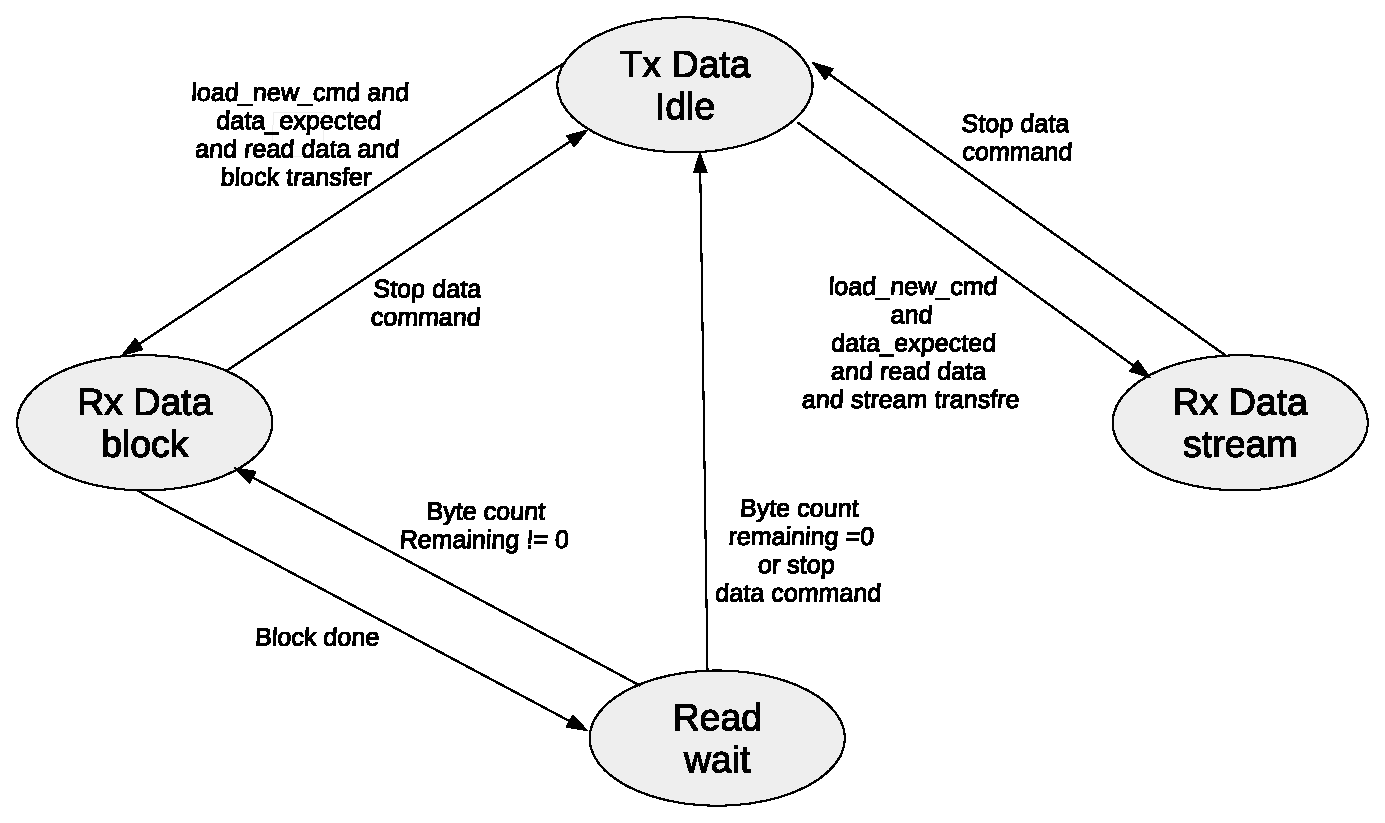
\includegraphics[width=0.5\textwidth]{./27-SDHOST/figures/rx_data_state_machine}
    \caption{Data Receive State Machine}
    \label{Figure:rx_data_state_machine}
\end{figure}

\section{Software Restrictions for Proper CIU Operation}
\begin{itemize}
	\item Only one card at a time can be selected to execute a command or data transfer. For example, when data are being transferred to or from a card, a new command must not be issued to another card. A new command, however, can be issued to the same card, allowing it to read the device status or stop the transfer.
	\item Only one command at a time can be issued for data transfers.
	\item During an open-ended card-write operation, if the card clock is stopped due to FIFO being empty, the software must fill FIFO with data first, and then start the card clock. Only then can it issue a stop/abort command to the card.
	\item During an SDIO/COMBO card transfer, if the card function is suspended and the software wants to resume the suspended transfer, it must first reset FIFO, and then issue the resume command as if it were a new data-transfer command.
	\item When issuing card reset commands (CMD0, CMD15 or CMD52\_reset), while a card data transfer is in progress, the software must set the stop\_abort\_cmd bit in the Command register, so that the CIU can stop the data transfer after issuing the card reset command.
	\item When the data's end bit error is set in the RINTSTS register, the CIU does not guarantee SDIO interrupts. In such a case, the software ignores SDIO interrupts and issues a stop/abort command to the card, so that the card stops sending read-data.
    \item If the card clock is stopped due to FIFO being full during a card read, the software will read at least two FIFO locations to restart the card clock.
	\item Only one CE-ATA device  at a time can be selected for a command or data transfer. For example, when data are transferred from a CE-ATA device, a new command should not be sent to another CE-ATA device.
	\item If a CE-ATA device's interrupts are enabled (nIEN=0), a new RW\_BLK command should not be sent to the same device if the execution of a RW\_BLK command is already in progress (the RW\_BLK command used in this databook is the RW\_MULTIPLE\_BLOCK MMC command defined by the CE-ATA specifications). Only the CCSD can be sent while waiting for the CCS.
	\item If, however, a CE-ATA device's interrupts are disabled (nIEN=1), a new command can be issued to the same device, allowing it to read status information.
	\item Open-ended transfers are not supported in CE-ATA devices.
	\item The send\_auto\_stop signal is not supported (software should not set the send\_auto\_stop bit) in CE-ATA transfers.
\end{itemize}

After configuring the command start bit to 1, the values of the following registers cannot be changed before a command has been issued:

\begin{itemize}
	\item CMD -     command
	\item CMDARG -  command argument
	\item BYTCNT -  byte count
	\item BLKSIZ -  block size
	\item CLKDIV -  clock divider
	\item CKLENA -  clock enable
	\item CLKSRC -  clock source
	\item TMOUT -   timeout
	\item CTYPE -   card type
\end{itemize}

\section{RAM for Receiving and Sending Data}

The submodule RAM is a buffer area for sending and receiving data. It can be divided into two units: the one is for sending data, and the other is for receiving data. The process of sending and receiving data can also be achieved by the CPU and DMA for reading and writing. The latter method is described in detail in Section \ref{linkedlist}.

\subsection{Transmit RAM Module}
There are two ways to enable a write operation: DMA and CPU read/write.

If SDIO-sending is enabled, data can be written to the transferred RAM module by APB interface or DMA. Data will be written from register EMAC\_FIFO to the CPU, directly, by an APB interface.

\subsection{Receive RAM Module}

There are two ways to enable a read operation: DMA and CPU read/write.

When a subunit of the data path receives data, the subdata will be written onto the receive-RAM. Then, these subdata can be read either with the APB or the DMA method at the reading end. Register EMAC\_FIFO can be read by the APB directly.

\section{Descriptor Chain}
Each linked list module consists of two parts: the linked list itself and a data buffer. In other words, each module points to a unique data buffer and the linked list that follows the module. Figure \ref{Figure:Chain_Descriptor} shows the descriptor chain.

\begin{figure}[H]
    \centering
    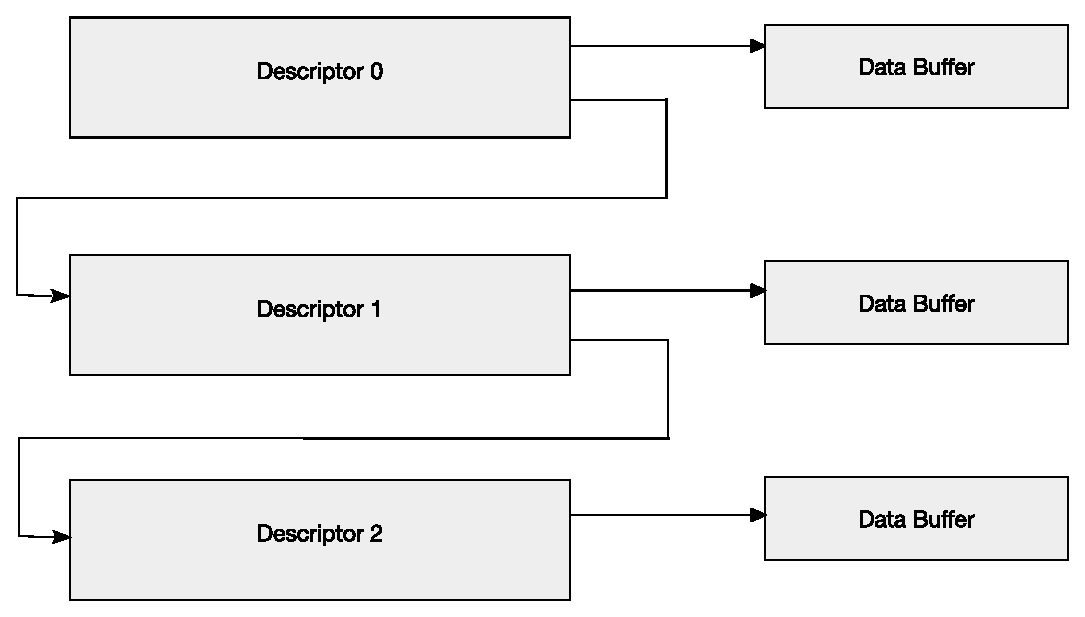
\includegraphics[width=0.7\textwidth]{./27-SDHOST/figures/Chain_Descriptor}
    \caption{Descriptor Chain}
    \label{Figure:Chain_Descriptor}
\end{figure}

\section{The Structure of a Linked List}\label{linkedlist}
Each linked list consists of four words. As is shown below, Figure \ref{Figure:Descriptor} demonstrates the linked list's structure, and Table \ref{DES0}, Table \ref{DES1}, Table \ref{DES2}, Table \ref{DES3} provide the descriptions of linked lists.

\begin{figure}[H]
    \centering
    
\includegraphics[width=0.7\textwidth]{./27-SDHOST/figures/Descriptor}
    \caption{The Structure of a Linked List}
    \label{Figure:Descriptor}
\end{figure}

The DES0 element contains control and status information.

\begin{longtable}[c]{ |p{3cm}|p{4cm}|p{8cm}| }
\caption{DES0} \label{DES0}\\
\hline
\rowcolor{lightgray}
Bits &Name & Description \\
\hline
\endfirsthead
\hline
\rowcolor{lightgray}
Bits &Name & Description  \\
\hline
\endhead
\endfoot
\multirow{4}{*}{31} & \multirow{4}{*}{OWN} & When set, this bit indicates that the descriptor is owned by the DMAC. When reset, it indicates that the descriptor is owned by the Host. The DMAC clears this bit when it completes the data transfer.\\\hline
\multirow{11}{*}{30} & \multirow{11}{*}{CES (Card Error Summary)} & These error bits indicate the status of the transition to or from the card. \\
 & & The following bits are also present in RINTSTS, which indicates their digital logic OR gate.
 \begin{itemize}
     \item{EBE: End Bit Error}
     \item{RTO: Response Time out}
     \item{RCRC: Response CRC}
     \item{SBE: Start Bit Error}
     \item{DRTO: Data Read Timeout}
     \item{DCRC: Data CRC for Receive}
     \item{RE: Response Error}
 \end{itemize}\vspace{-1.5em}
 \\\hline
29:6 & Reserved & Reserved	\\\hline
\multirow{4}{*}{5} &\multirow{4}{*}{ER (End of Ring)} & When set, this bit indicates that the descriptor list has reached its final descriptor. The DMAC then returns to the base address of the list, creating a Descriptor Ring. \\\hline
\multirow{3}{*}{4} &\multirow{3}{*}{\makecell[l]{CH\\ (Second Address Chained)}} & When set, this bit indicates that the second address in the descriptor is the Next Descriptor address. When this bit is set, BS2 (DES1[25:13]) should be all zeros. \\\hline
\multirow{4}{*}{3} & \multirow{4}{*}{FD (First Descriptor)}& When set, this bit indicates that this descriptor contains the first buffer of the data. If the size of the first buffer is 0, the Next Descriptor contains the beginning of the data. \\\hline
\multirow{7}{*}{2} & \multirow{7}{*}{LD (Last Descriptor)}&  This bit is associated with the last block of a DMA transfer. When set, the bit indicates that the buffers pointed by this descriptor are the last buffers of the data. After this descriptor is completed, the remaining byte count is 0. In other words, after the descriptor with the LD bit set is completed, the remaining byte count should be 0.\\\hline
\multirow{3}{*}{1}&\multirow{3}{*}{\makecell[l]{DIC (Disable Interrupt\\ on Completion)}}& When set, this bit will prevent the setting of the TI/RI bit of the DMAC Status Register (IDSTS) for the data that ends in the buffer pointed by this descriptor. \\\hline
0 & Reserved& Reserved \\\hline
\end{longtable}

The DES1 element contains the buffer size.
\begin{longtable}[c]{ |p{3cm}|p{4cm}|p{8cm}| }
\caption{DES1} \label{DES1}\\
\hline
\rowcolor{lightgray}
Bits &Name & Description \\
\hline
\endfirsthead
\hline
\rowcolor{lightgray}
Bits &Name & Description  \\
\hline
\endhead
\endfoot

31:26 & Reserved& Reserved  \\\hline
25:13 & Reserved& Reserved  \\\hline
\multirow{4}{*}{12:0}  & \multirow{4}{*}{BS1 (Buffer 1 Size)} &  Indicates the data buffer byte size, which must be a multiple of four. In the case where the buffer size is not a multiple of four, the resulting behavior is undefined. This field should not be zero.    \\\hline

\end{longtable}

The DES2 element contains the address pointer to the data buffer.\\

\begin{longtable}[c]{ |p{3cm}|p{4cm}|p{8cm}| }
\caption{DES2} \label{DES2}\\
\hline
\rowcolor{lightgray}
Bits &Name & Description \\
\hline
\endfirsthead
\hline
\rowcolor{lightgray}
Bits &Name & Description  \\
\hline
\endhead
\endfoot
\multirow{2}{*}{31:0}& \multirow{2}{*}{Buffer Address Pointer 1} & These bits indicate the physical address of the data buffer.    \\\hline

\end{longtable}

The DES3 element contains the address pointer to the next descriptor if the present descriptor is not the last one in a chained descriptor structure.
\vspace{-1em}

\begin{longtable}[c]{ |p{3cm}|p{4cm}|p{8cm}| }
\caption{DES3} \label{DES3}\\
\hline
\rowcolor{lightgray}
Bits &Name & Description \\
\hline
\endfirsthead
\hline
\rowcolor{lightgray}
Bits &Name & Description  \\
\hline
\endhead
\endfoot
\multirow{5}{*}{31:0}& \multirow{5}{*}{Next Descriptor Address} &  If the Second Address Chained (DES0[4]) bit is set, then this address contains the pointer to the physical memory where the Next Descriptor is present.\\
&&If this is not the last descriptor, then the Next Descriptor address pointer must be DES3[1:0] = 0.    \\\hline
\end{longtable}

\section{Initialization}
\subsection{DMAC Initialization}
The DMAC initialization should proceed as follows:
\begin{itemize}
\item  Write to the DMAC Bus Mode Register (BMOD\_REG) will set the Host bus's access parameters.
\item Write to the DMAC Interrupt Enable Register (IDINTEN) will mask any unnecessary interrupt causes.
\item The software driver creates either the transmit or the receive descriptor list. Then, it writes to the DMAC Descriptor List Base Address Register (DBADDR), providing the DMAC with the starting address of the list.
\item The DMAC engine attempts to acquire descriptors from descriptor lists.
\end{itemize}

\subsection{DMAC Transmission Initialization}
The DMAC transmission occurs as follows:

\begin{enumerate}
\item The Host sets up the elements (DES0-DES3) for transmission, and sets the OWN bit (DES0[31]). The Host also prepares the data buffer.
\item The Host programs the write-data command in the CMD register in BIU.
\item The Host also programs the required transmit threshold  (TX\_WMARK field in FIFOTH register).
\item The DMAC engine fetches the descriptor and checks the OWN bit. If the OWN bit is not set, it means that the host owns the descriptor. In this case, the DMAC enters a suspend-state and asserts the Descriptor Unable interrupt in the IDSTS register. In such a case, the host needs to release the DMAC by writing any value to PLDMND\_REG.
\item It then waits for the Command Done (CD) bit and no errors from BIU, which indicates that a transfer can be done.
\item Subsequently, the DMAC engine waits for a DMA interface request (dw\_dma\_req) from BIU. This request will be generated, based on the programmed transmit-threshold value. For the last bytes of data which cannot be accessed using a burst, single transfers are performed on the AHB Master Interface.
\item The DMAC fetches the transmit data from the data buffer in the Host memory and transfers them to FIFO for transmission to card.
\item When data span across multiple descriptors, the DMAC fetches the next descriptor and extends its operation using the following descriptor. The last descriptor bit indicates whether the data span multiple descriptors or not.
\item When data transmission is complete, the status information is updated in the IDSTS register by setting the Transmit Interrupt, if it has already been enabled. Also, the OWN bit is cleared by the DMAC by performing a write transaction to DES0.
\end{enumerate}

\subsection{DMAC Reception Initialization}
The DMAC  reception occurs as follows:

\begin{enumerate}
\item The Host sets up the element (DES0-DES3) for reception, and sets the OWN bit (DES0[31]).
\item The Host programs the read-data command in the CMD register in BIU.
\item Then, the Host programs the required level of the receive-threshold (RX\_WMARK field in FIFOTH register).
\item The DMAC engine fetches the descriptor and checks the OWN bit. If the OWN bit is not set, it means that the host owns the descriptor. In this case, the DMA enters a suspend-state and asserts the Descriptor Unable interrupt in the IDSTS register. In such a case, the host needs to release the DMAC by writing any value to PLDMND\_REG.
\item It then waits for the Command Done (CD) bit and no errors from BIU, which indicates that a transfer can be done.
\item The DMAC engine then waits for a DMA interface request (dw\_dma\_req) from BIU. This request will be generated, based on the programmed receive-threshold value. For the last bytes of the data which cannot be accessed using a burst, single transfers are performed on the AHB.
\item The DMAC fetches the data from FIFO and transfers them to the Host memory.
\item When data span across multiple descriptors, the DMAC will fetch the next descriptor and extend its operation using the following descriptor. The last descriptor bit indicates whether the data span multiple descriptors or not.
\item When data reception is complete, the status information is updated in the IDSTS register by setting Receive-Interrupt, if it has already been enabled. Also, the OWN bit is cleared by the DMAC by performing a write-transaction to DES0.
\end{enumerate}

\section{SD/MMC Timing}

Figure \ref{fig:sdmmc-timing} shows the timing diagram for SD/MMC in high-speed (HS) mode. Table \ref{tab:sdmmc-timing} lists the timing requirements. These requirements are crucial for ensuring reliable and synchronized data communication in HS mode.

\begin{figure}[h]
    \centering
    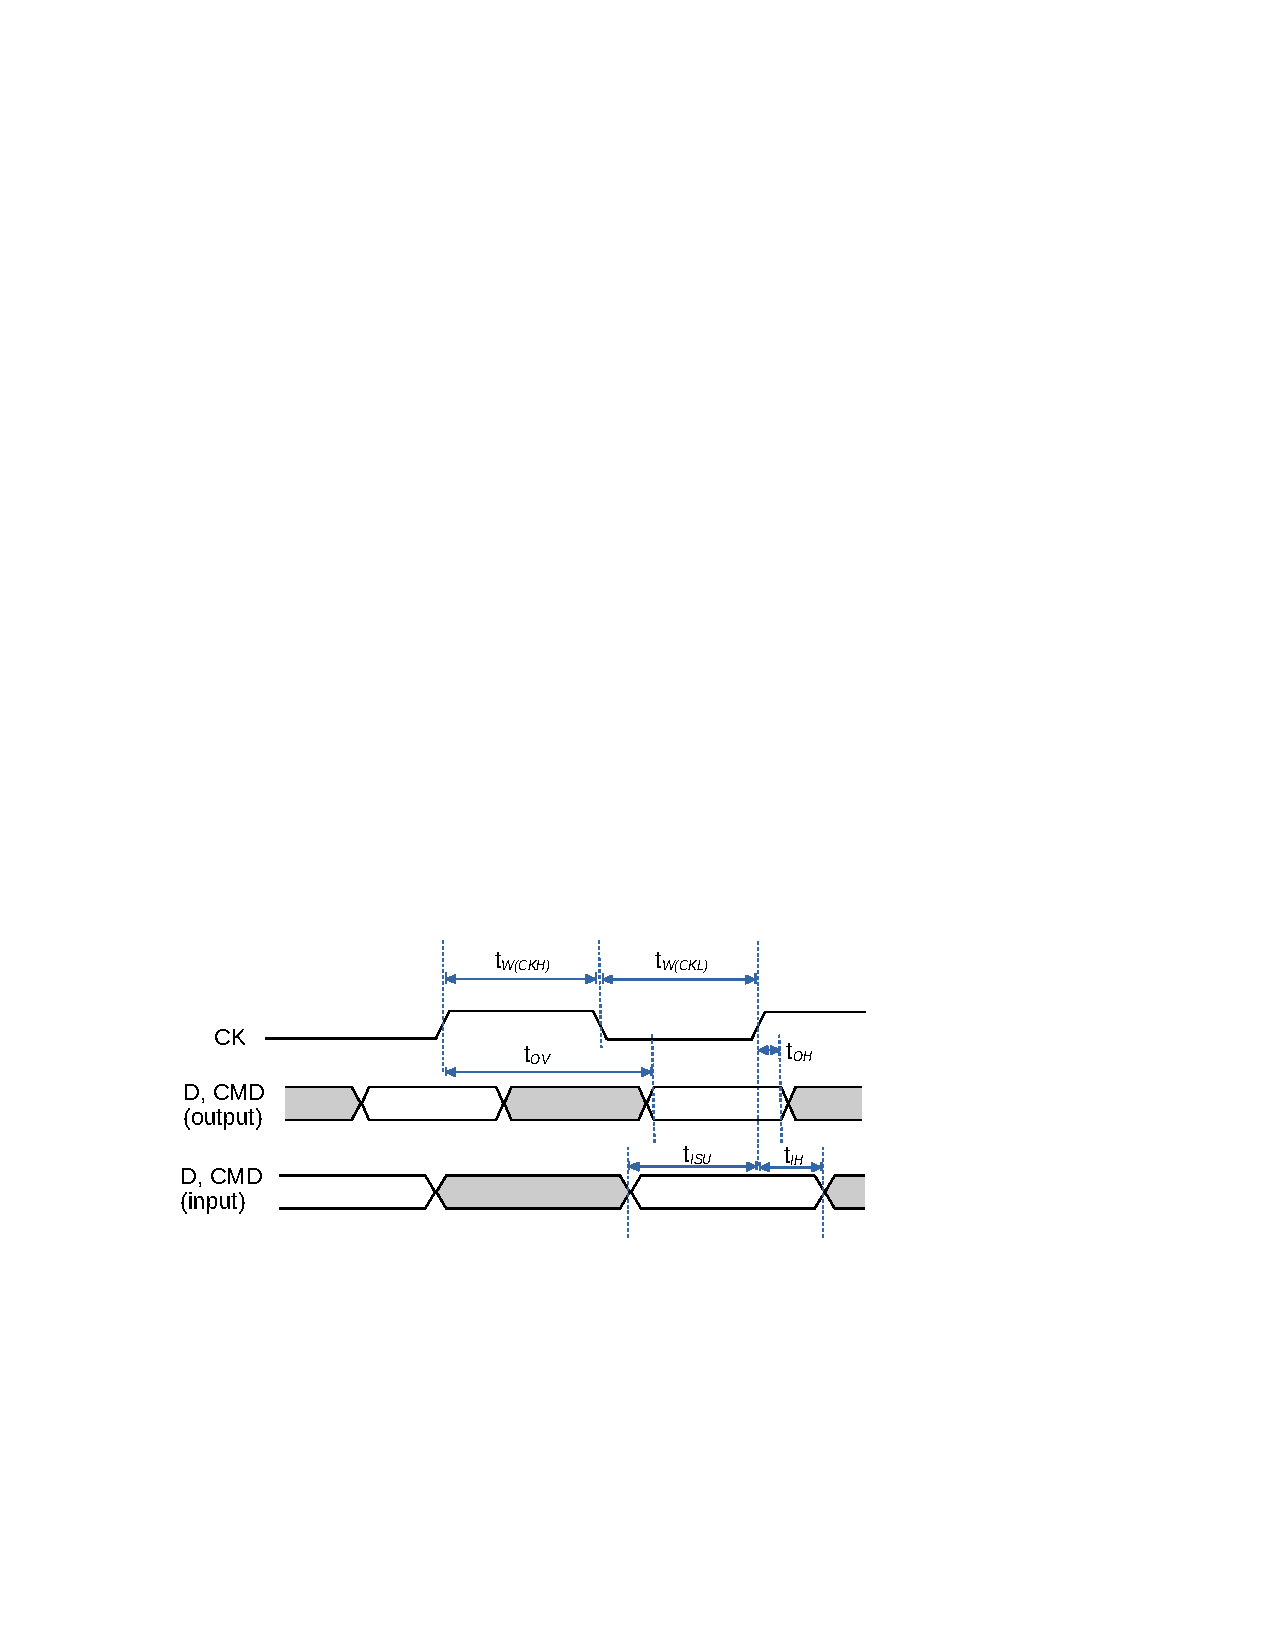
\includegraphics[width=0.7\textwidth]{./27-SDHOST/figures/esp32-sdmmc-timing}
    \caption{SD/MMC Timing in HS Mode}\label{fig:sdmmc-timing}
\end{figure}

\begin{longtable}[c]{|l|l|l|r|r|r|c|}
    \caption{SD/MMC Timing Requirements}
    \label{tab:sdmmc-timing}
    \\\hline
    \rowcolor{lightgray}
\textbf{Symbol} & \textbf{Parameter} & \textbf{Conditions} & \textbf{Min} & \textbf{Typ} & \textbf{Max} & \textbf{Unit} \\\hline
t$_{W(CKL)}$ & Clock Low Time & f$_{PP}$ = 80 MHz & 11.5 & 12.5 & --- & ns \\\hline
t$_{W(CKH)}$ & Clock High Time & f$_{PP}$ = 80 MHz & 11.5 & 12.5 & --- & ns \\\hline
t$_{ISU}$ & Input Setup Time in HS Mode & f$_{PP}$ = 80 MHz & 3.4 & --- & --- & ns \\\hline
t$_{IH}$ & Input Hold Time in HS Mode & f$_{PP}$ = 80 MHz & 1.1 & --- & --- & ns \\\hline
t$_{OV}$ & Output Valid Time in HS Mode & f$_{PP}$ = 80 MHz & --- & --- & 5.9 & ns \\\hline
t$_{OH}$ & Output Hold Time in HS Mode & f$_{PP}$ = 80 MHz & 0.5 & --- & --- & ns \\\hline
\end{longtable}

\textbf{Legend:}

\begin{itemize}
    \item f$_{PP}$ - Clock frequency in data transfer mode.
    \item t$_{W(CKL)}$/t$_{W(CKH)}$ - Clock Low/High Time: t$_{W(CKL)}$/t$_{W(CKH)}$ represents the time that the clock signal (CK) should remain in the low or high state.
    \item t$_{ISU}$ - Input Setup Time in HS Mode: t$_{ISU}$ represents the setup time required for CMD and D (data lines) inputs.
    \item t$_{IH}$ - Input Hold Time in HS Mode: t$_{IH}$ specifies the hold time required for CMD and D inputs.
    \item t$_{OV}$ - Output Valid Time in HS Mode: t$_{OV}$ defines the time it takes for the CMD and D outputs to be ready.
    \item t$_{OH}$ - Output Hold Time in HS Mode: t$_{OH}$ specifies the hold time required for the CMD and D outputs to be valid.
    \item The timing of the CMD and D inputs and outputs are measured in relation to the clock signal CK.
\end{itemize}

\section{Clock Phase Selection}\label{sdmmc_phase_sel}
If the setup time requirements for the input or output data signal are not met, users can specify the clock phase, as shown in the figure below.
\begin{figure}[H]
    \centering
    \fbox{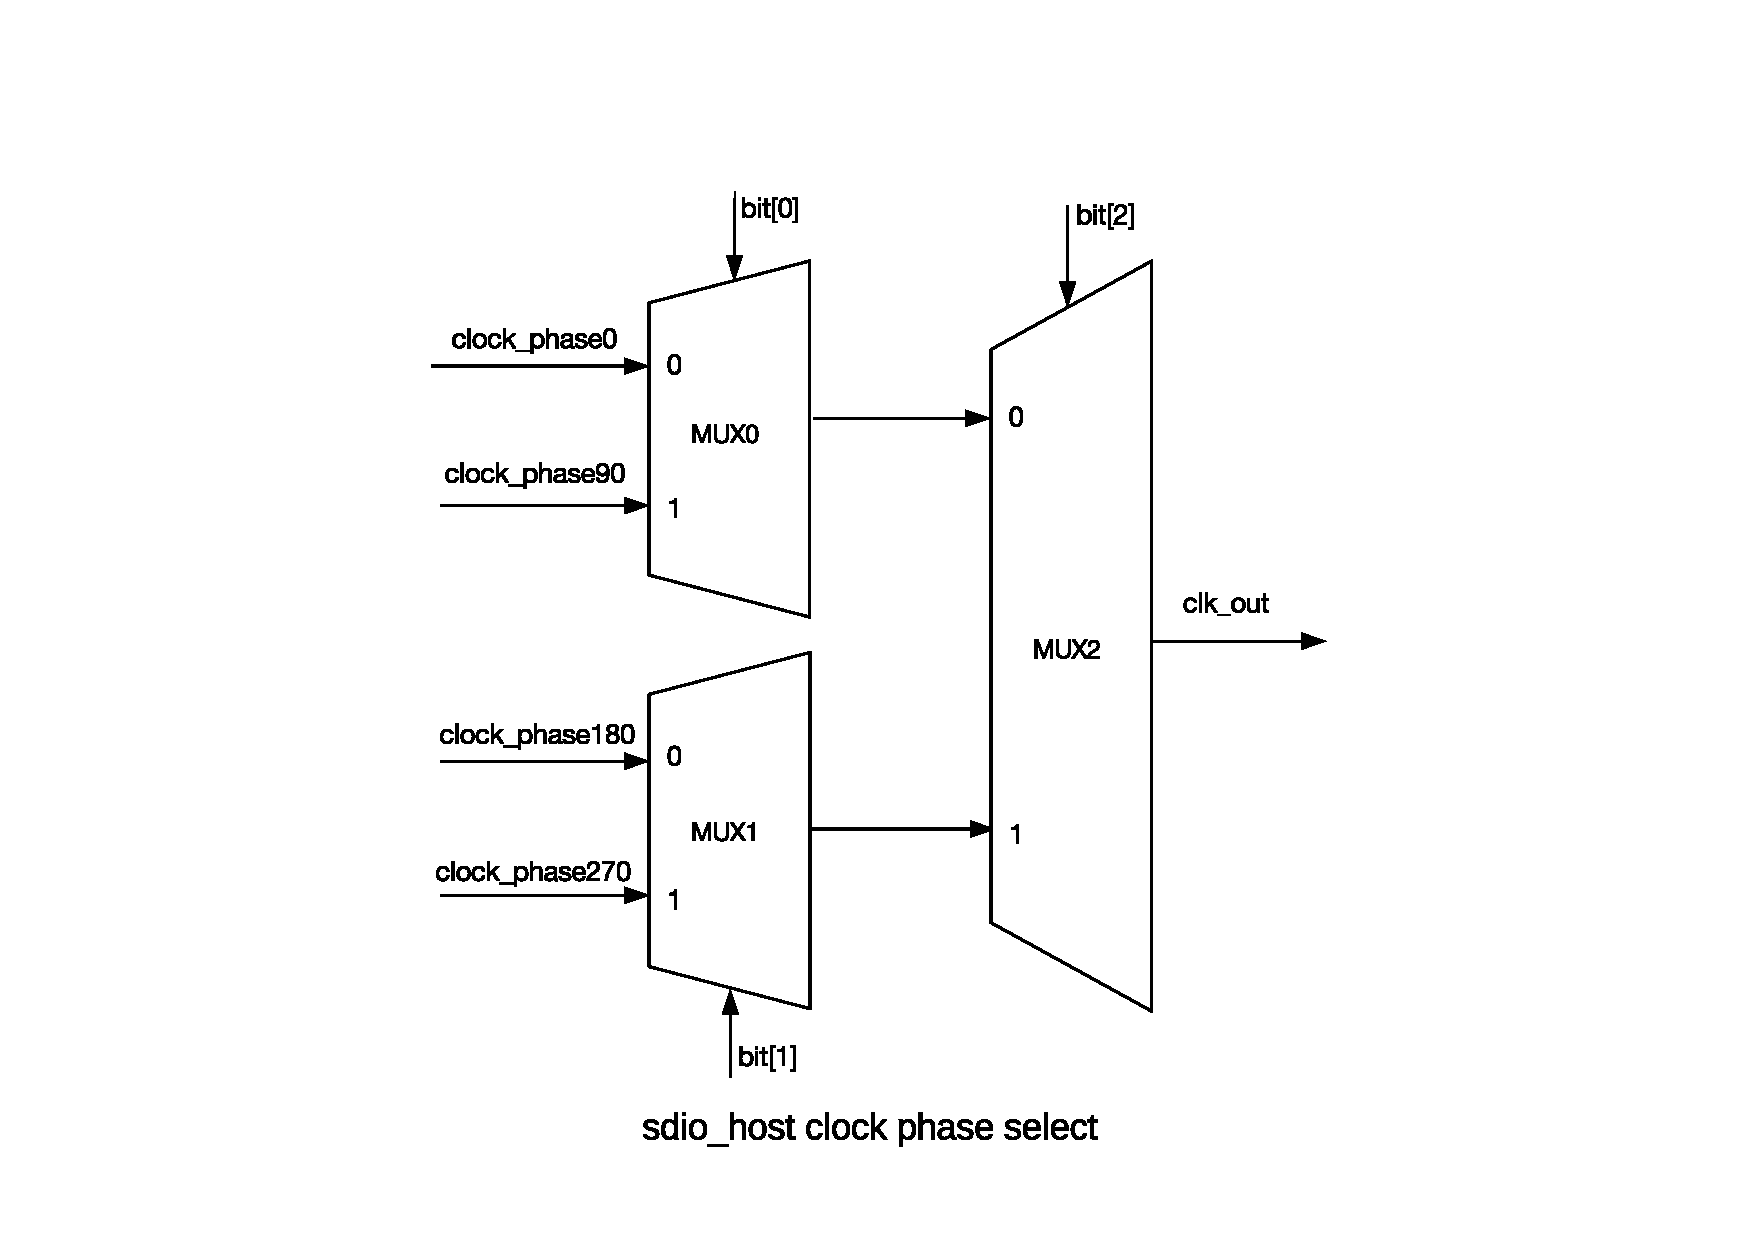
\includegraphics[width=0.7\textwidth]{./27-SDHOST/figures/sdmmc_phase_sel}}
    \caption{Clock Phase Selection}
\end{figure}

Please find detailed information on the clock phase selection register \hyperref[regdesc:CLKEDGESEL]{CLK\_EDGE\_SEL} in Section Registers.

\section{Interrupt}
Interrupts can be generated as a result of various events. The IDSTS register contains all the bits that might cause an interrupt. The IDINTEN register contains an enable bit for each of the events that can cause an interrupt.

There are two groups of summary interrupts, "Normal" ones (bit8 NIS) and "Abnormal" ones (bit9 AIS), as outlined in the IDSTS register. Interrupts are cleared by writing 1 to the position of the corresponding bit. When all the enabled interrupts within a group are cleared, the corresponding summary bit is also cleared. When both summary bits are cleared, the interrupt signal dmac\_intr\_o is de-asserted (stops signalling).

Interrupts are not queued up, and if a new interrupt-event occurs before the driver has responded to it, no additional interrupts are generated. For example, the Receive Interrupt IDSTS[1] indicates that one or more data were transferred to the Host buffer.

An interrupt is generated only once for concurrent events. The driver must scan the IDSTS register for the interrupt cause.

\hypertarget{sdhost-reg-summ}{}
\section{Register Summary}

The addresses in this section are relative to the SD/MMC base address provided in Table \ref{table:Peripheral_Address_Mapping} in Chapter \ref{mod:sysmem} \textit{\nameref{mod:sysmem}}.

The abbreviations given in Column \textbf{Access} are explained in Section \hyperref[glossary-access-types]{\textit{Access Types for Registers}}.


\subfile{\modulefiles/sdmmc_reg_summary_en.tex}

\section{Registers}

SD/MMC controller registers can be accessed by the APB bus of the CPU.

The addresses in this section are relative to the SD/MMC base address provided in Table \ref{table:Peripheral_Address_Mapping} in Chapter \ref{mod:sysmem} \textit{\nameref{mod:sysmem}}.

For how to program reserved fields, please refer to Section \hyperref[programming-reserved-field]{\textit{Programming Reserved Register Field}}.


\subfile{\modulefiles/sdmmc_reg_en.tex}
\end{document}
